% Options for packages loaded elsewhere
\PassOptionsToPackage{unicode}{hyperref}
\PassOptionsToPackage{hyphens}{url}
%
\documentclass[
]{article}
\title{Caso de estudio \#1: Tiempo de falla}
\author{Sergio Andres Niño Marin, Sergio Andres Gerena Gomez}
\date{26/sept/2022}

\usepackage{amsmath,amssymb}
\usepackage{lmodern}
\usepackage{iftex}
\ifPDFTeX
  \usepackage[T1]{fontenc}
  \usepackage[utf8]{inputenc}
  \usepackage{textcomp} % provide euro and other symbols
\else % if luatex or xetex
  \usepackage{unicode-math}
  \defaultfontfeatures{Scale=MatchLowercase}
  \defaultfontfeatures[\rmfamily]{Ligatures=TeX,Scale=1}
\fi
% Use upquote if available, for straight quotes in verbatim environments
\IfFileExists{upquote.sty}{\usepackage{upquote}}{}
\IfFileExists{microtype.sty}{% use microtype if available
  \usepackage[]{microtype}
  \UseMicrotypeSet[protrusion]{basicmath} % disable protrusion for tt fonts
}{}
\makeatletter
\@ifundefined{KOMAClassName}{% if non-KOMA class
  \IfFileExists{parskip.sty}{%
    \usepackage{parskip}
  }{% else
    \setlength{\parindent}{0pt}
    \setlength{\parskip}{6pt plus 2pt minus 1pt}}
}{% if KOMA class
  \KOMAoptions{parskip=half}}
\makeatother
\usepackage{xcolor}
\IfFileExists{xurl.sty}{\usepackage{xurl}}{} % add URL line breaks if available
\IfFileExists{bookmark.sty}{\usepackage{bookmark}}{\usepackage{hyperref}}
\hypersetup{
  pdftitle={Caso de estudio \#1: Tiempo de falla},
  pdfauthor={Sergio Andres Niño Marin, Sergio Andres Gerena Gomez},
  hidelinks,
  pdfcreator={LaTeX via pandoc}}
\urlstyle{same} % disable monospaced font for URLs
\usepackage[margin=1in]{geometry}
\usepackage{graphicx}
\makeatletter
\def\maxwidth{\ifdim\Gin@nat@width>\linewidth\linewidth\else\Gin@nat@width\fi}
\def\maxheight{\ifdim\Gin@nat@height>\textheight\textheight\else\Gin@nat@height\fi}
\makeatother
% Scale images if necessary, so that they will not overflow the page
% margins by default, and it is still possible to overwrite the defaults
% using explicit options in \includegraphics[width, height, ...]{}
\setkeys{Gin}{width=\maxwidth,height=\maxheight,keepaspectratio}
% Set default figure placement to htbp
\makeatletter
\def\fps@figure{htbp}
\makeatother
\setlength{\emergencystretch}{3em} % prevent overfull lines
\providecommand{\tightlist}{%
  \setlength{\itemsep}{0pt}\setlength{\parskip}{0pt}}
\setcounter{secnumdepth}{5}
\ifLuaTeX
  \usepackage{selnolig}  % disable illegal ligatures
\fi

\begin{document}
\maketitle

{
\setcounter{tocdepth}{2}
\tableofcontents
}
\hypertarget{caso-de-estudio}{%
\subsection*{Caso de estudio}\label{caso-de-estudio}}
\addcontentsline{toc}{subsection}{Caso de estudio}

Un investigador del Departamento de Ingeniería Electrónica y Eléctrica
de una universidad necesita analizar unos datos sobre los tiempos de
falla de un determinado tipo de alambre (Tipo 1). En este problema, el
tiempo de falla se define como el número de veces que una máquina podría
tensionar el alambre antes de romperse. Los siguientes datos
corresponden a \$ n= 14\$ tiempos de falla de una parte del experimento:
\[
495 \quad 541 \quad 1461 \quad 1555 \quad 1603 \quad 2201 \quad 2750 \quad 3468 \quad 3516 \quad 4319 \quad 6622 \quad 7728 \quad 13159 \quad 21194
\] A partir de este contexto, Su incertidumbre acerca de estos datos
antes de que fueran observados es intercambiable. Por lo tanto, resulta
apropiado modelar los datos como condicionalmente independientes e
idénticamente distribuidos. El modelo más simple para los datos del
tiempo de falla involucra la distribución Exponencial:
\begin{equation}\label{exponential-model-1}
    y_i \mid \lambda \stackrel{ \mbox{\footnotesize iid} }{ \sim } \textsf{Exp} ( \lambda )\text{,} \ \ \ \textrm{i.e.,} \ \ \ p( y_i \mid \lambda ) = \frac{ 1 }{ \lambda }\, \exp{\left( - \frac{y_i }{ \lambda }\right) } \quad\text{para $y_i > 0$ y $\lambda > 0$, con $i=1,\ldots,n$.} 
\end{equation}

\hypertarget{pregunta-1}{%
\subsection*{Pregunta 1}\label{pregunta-1}}
\addcontentsline{toc}{subsection}{Pregunta 1}

Muestre que \(s=\sum_{i=1}^n y_i\) es un estadístico suficiente para
\(\lambda\).

\hypertarget{solucion}{%
\subsubsection*{Solucion:}\label{solucion}}
\addcontentsline{toc}{subsubsection}{Solucion:}

Aplicando el criterio de factorizacion de Fisher-Neyman se observa que:
\[
\begin{split}
\mathcal{L}(\lambda|y_1,...,y_n)&=\prod_{i=1}^{n}\frac{1}{\lambda}e^{-\frac{y_i}{\lambda}}I_{(0,\infty)}(y_i)\\
&=\underbrace{\frac{1}{\lambda^n}e^{-\frac{\sum_{i=1}^ny_i}{\lambda}}}_{g(T(y),\lambda)}\overbrace{\prod_{i=1}^{n}I_{(0,\infty)}(y_i)}^{h(y)} \\
\end{split}
\] Con esto, vemos que un estadistico suficiente es
\(s=\sum_{i=1}^ny_i\) dado que este estadistico cumple al poderse
factorizar de la expresion de verosimilitud en una funcion g que solo
depende del estadistico suficiente y el parametro.

\hypertarget{pregunta-2}{%
\subsection*{Pregunta 2}\label{pregunta-2}}
\addcontentsline{toc}{subsection}{Pregunta 2}

Se dice que la variable aleatoria \(X\) tiene distribución Gamma-Inversa
con parámetros \(\alpha>0\) y \(\beta>0\), si la función de densidad de
\(X\) está dada por: \[
    X \sim \textsf{GI} ( \alpha, \beta )\text{,} \ \ \ \textrm{i.e.,} \ \ \ 
    p ( x ) = \frac{ \beta^\alpha }{ \Gamma ( \alpha ) } x^{ - ( \alpha + 1 ) } \exp{ \left( - \frac{ \beta }{ x } \right) } \quad\text{para $x>0$}.
    \] Muestre que si \(X\sim\textsf{Gamma}(\alpha,\beta)\), entonces
\(\frac{1}{X}\sim \textsf{GI} ( \alpha, \beta )\).

\hypertarget{solucion-1}{%
\subsubsection*{Solucion:}\label{solucion-1}}
\addcontentsline{toc}{subsubsection}{Solucion:}

Siendo \(X\) una V.a absolutamente continua, se usa el teorema de la
transformacion para determinar la distribucion de
\(Y=\frac{1}{X} \ con \ X>0\) a partir de la distribucion conocida \(X\)
\[
P\left( \frac{1}{X}\right) =f_X\left( \frac{1}{Y}\right) \left| \frac{\delta X}{\delta Y} \right|= \frac{\beta^{\alpha}}{\Gamma(\alpha)}\left(\frac{1}{Y} \right)^{\alpha -1}exp\left( -\frac{\beta}{Y} \right) \left| -\frac{1}{Y^2} \right|
\] Resolviendo como se indica a continuacion \[
\begin{split}
P\left( \frac{1}{X}\right) &=\frac{\beta^{\alpha}}{\Gamma(\alpha)}\left(\frac{1}{Y} \right)^{\alpha -1}exp\left( -\frac{\beta}{Y} \right) \left( \frac{1}{Y^2} \right)\\
&=\frac{\beta^{\alpha}}{\Gamma(\alpha)}\left(\frac{1}{Y} \right)^{\alpha +1}exp\left( -\frac{\beta}{Y} \right) \\
P\left( \frac{1}{X}\right)=P\left( Y \right)&=\frac{\beta^{\alpha}}{\Gamma(\alpha)}Y^{-(\alpha +1)}exp\left( -\frac{\beta}{Y} \right) \sim GI(\alpha,\beta)
\end{split}
\] Dado que lo obtenido al aplicar el teorema de transformacion fue la
distribucion descrita como Gamma inversa (\(GI\)) con los respectivos
parametros, podemos asegurar que la afirmacion propuesta en el punto
resulta verdadera.

\hypertarget{punto-3}{%
\subsection*{Punto 3}\label{punto-3}}
\addcontentsline{toc}{subsection}{Punto 3}

Considere la distribución previa
\(\lambda \sim \textsf{GI} ( \alpha, \beta )\) junto con la distribución
muestral \eqref{exponential-model-1}. Halle la distribución posterior de
\(\lambda\).

\hypertarget{solucion-2}{%
\subsubsection*{Solucion:}\label{solucion-2}}
\addcontentsline{toc}{subsubsection}{Solucion:}

Para esto se emplea el teorema de bayes para encontrar la distribucion
posterior de \(\lambda\) a partir de la distribucion muestral y la
distribucion previa.

\[
\begin{split}
p(\lambda | \vec{y}) &\propto p(\vec{y}|\lambda)p(\lambda)\\
&\propto \left[ \prod_{i=1}^n \frac{1}{\lambda}exp \left( \frac{-y_i}{\lambda} \right) \right] \frac{\beta^\alpha}{\Gamma(\alpha)}\lambda^{-(\alpha+1)}exp\left( -\frac{\beta}{\lambda} \right)\\
&\propto \lambda^{-n}exp\left( \frac{-1}{\lambda}\sum_{i=1}^ny_i \right)\lambda^{-(\alpha+1)}exp\left( \frac{-\beta}{\lambda} \right)\\
p(\lambda|\vec{y})&\propto \lambda^{-(\alpha +n +1)}exp\left( \frac{-(\beta + s)}{\lambda} \right) \sim GI(\alpha +n,\beta+s)
\end{split}
\]

\hypertarget{punto-4}{%
\subsection*{Punto 4}\label{punto-4}}
\addcontentsline{toc}{subsection}{Punto 4}

Se tiene información externa de otro experimento de acuerdo con el cual
la distribución previa de \(\lambda\) debería tener una media
\(\mu_0 = 4500\) y una desviación estándar \(\sigma_0 = 1800\). Haga un
gráfico de las distribuciones previa y posterior en el mismo gráfico.

\hypertarget{solucion-3}{%
\subsubsection*{Solucion:}\label{solucion-3}}
\addcontentsline{toc}{subsubsection}{Solucion:}

Lo primero es, encontrar los hiperparametros de la distribucion previa
tal que satisfaga la media \(\mu_0 = 4500\) y la desviacion estandar
\(\sigma_0 = 1800\), dando el siguiente sistema de ecuaciones: \[
\begin{split}
4500&=\frac{\beta_0}{\alpha_0-1}\ \ \ \ \ \ \ para \ \alpha_0 >1\\
1800&=\sqrt{\frac{\beta_0^2}{(\alpha_0-1)^2(\alpha_0-2)}} \ \ \ \ \ \ \ para \ \alpha_0>2
\end{split}
\]

Resolviendo el sistema de ecuaciones, tenemos que \(\alpha_0=8.25\) y
\(\beta_0=32625\). con esto ya se puede construir la distribucion
previa.

Ahora, en base al punto anterior donde se calculo la distribucion
posterior para este modelo sigue la forma \(GI(\alpha +n, \beta +s)\)
donde \(n\) es el tamaño de la muestra y \(s\) es la suma de todos los
\(y_i\). Empleando una suma sobre los 14 terminos que se tiene en los
datos, resulta que \(n=14\) y \(s=70612\).

Ahora sigue construir y graficar ambas distribuciones, tanto la previa
como la posterior, usando codigo en R para realizar dicha accion, el
resultado es el observado a continuacion

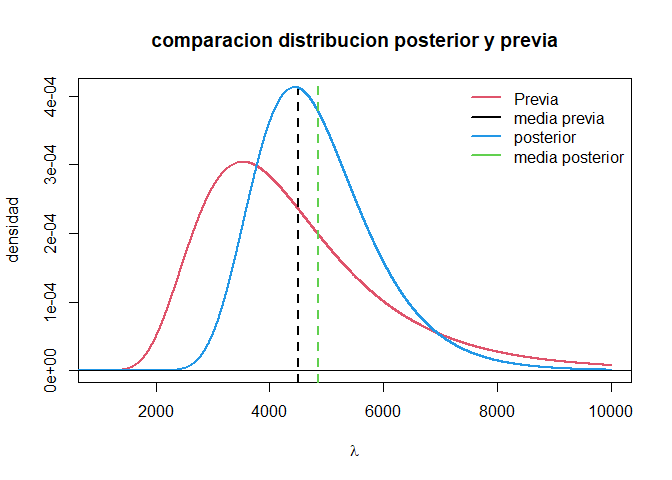
\includegraphics{bayes-parcial1-Sergio-Andrés-Niño-Marín-Sergio-Andres-Gerena-Gomez_files/figure-latex/unnamed-chunk-1-1.pdf}

\hypertarget{punto-5}{%
\subsection*{Punto 5}\label{punto-5}}
\addcontentsline{toc}{subsection}{Punto 5}

Halle el estimador de máxima verosimilitud (MLE, por sus siglas en
inglés) de \(\lambda\).

\hypertarget{solucion-4}{%
\subsubsection*{Solucion:}\label{solucion-4}}
\addcontentsline{toc}{subsubsection}{Solucion:}

Para encontrar el estimador de maxima verosimilitud, lo primero es
calcular la funcion de verosimilitud del parametro dada la muestra y a
dicha funcion se le encuentra el maximo global, pero antes, se usa la
parametrizacion de la exponencial donde \(\theta=\frac{1}{\lambda}\),
luego de encontrar el MLE para dicho parametro, se emplea la invarianza
funcional del estimador MLE para encontrar el estimador MLE de
\(\lambda\).

Se empieza encontrando la funcion de verosimilitud del parametro
\(\theta\) de la siguiente manera \[
\begin{split}
\mathcal{L}(\theta|\vec{y})&=\prod_{i=1}^np(y_i|\theta)\\
&=\prod_{i=1}^n\theta e^{-\theta y_i}\\
&=\theta^ne^{-\theta\sum_{i=1}^ny_i}
\end{split}
\] Para simplificar la notacion y tambien las matematicas en los
siguientes pasos , se usa como convencion que \(s=\sum_{i=1}^n\) ademas
de que en el proceso de maximizacion se emplea la funcion
log-verosimilitud \(\mathcal{l}(\theta|\vec{y})\) la cual es el
logaritmo natural de la anteriormente encontrada.

Siguiendo con la maximisacion de la funcion, primero se encuentran los
puntos criticos empleando la primera derivada \[
\begin{split}
\frac{\delta}{\delta\theta}l(\theta|\vec{y})&=\frac{\delta}{\delta \theta}\left( \right)n*ln(\theta)
\end{split}
\] \#\# Github Markdown

To get github friendly Markdown document for cleanly tracking changes to
document in Github, put the following output first:

\begin{verbatim}
output:
  md_document:
    variant: "markdown_github"
\end{verbatim}

NOTE: You need to run this \textbf{LAST} though, since knitting other
formats wipes out the \texttt{test\_files} directory. To return to the
Knit button having other options (HTML, PDF, Word), move this output
type below the first option.

\hypertarget{references}{%
\subsection*{References}\label{references}}
\addcontentsline{toc}{subsection}{References}

\textless!-- placeholder for References in toc --!\textgreater{}

\end{document}
